\chapter{Application to blinking Eye simulation}
\label{chap_eye}

\section{Introduction}

The tear film is a thin layer of liquid film on the ocular surface spread through blinking. It serves several vital functions including protecting the ocular surface with moisture, transporting waste, and as providing a smooth ocular surface. Within each blink cycle, a tear film that is functioning properly will maintain a balance between tear secretion and loss. \cite{holly1977tear}.

	Dry eye syndrome (DES) is a collection of symptoms that include blurred vision, burning, foreign body sensation, and tearing and inflammation of the ocular surface. According to a study from 2007, an estimated 4.91 million Americans suffer from DES \cite{bron2007methodologies}. A malfunctioning or deficient tear film is thought to be a cause of DES \cite{nelson2011international}, causing the ocular tear film comunity to take interest in the function of the tear film \cite{johnson2004changes} as well as the connection between DES and tear film volume, evaporation \cite{bron2007methodologies}.
	
\begin{figure}
  \centering
  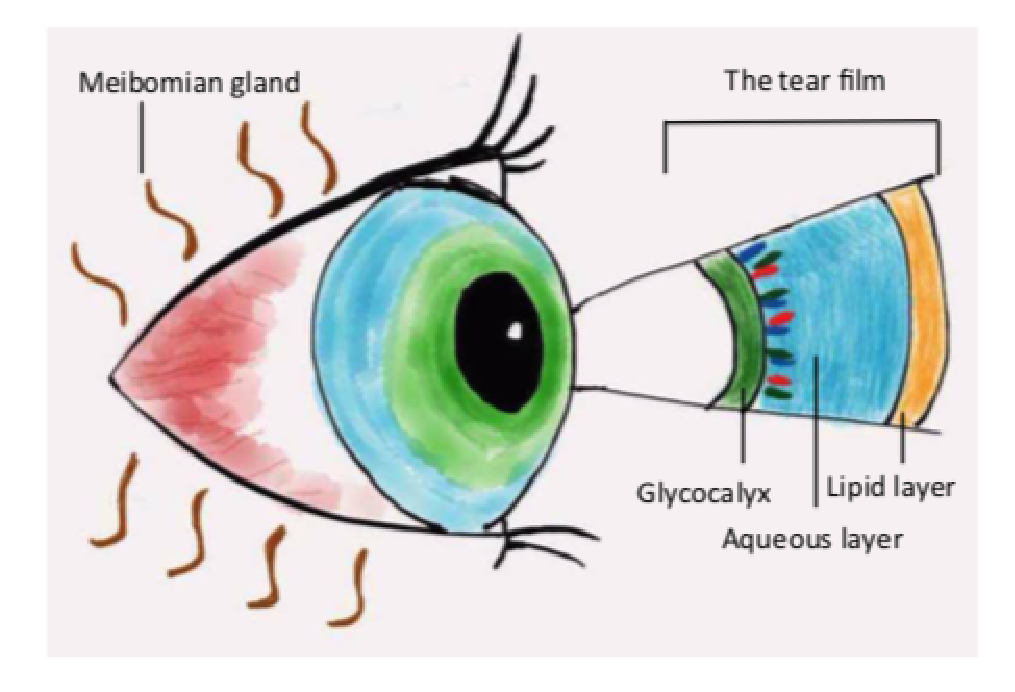
\includegraphics[scale=0.6]{Chapter4/eye_model.eps}
  \caption{Illustration of tear film with labeled layers \cite{zhong2018dynamics}.}
  \label{eye_levels}
\end{figure}

	The tear film is composed of three layers, as shown in Figure~\ref{eye_levels}. The anterior surface in contact with the air is an oily lipid layer which helps reduce evaporation \cite{norn1979semiquantitative,mishima1961oily}. The middle aqueous layer is composed mostly of water, and serves to lubricate the eye, move particles and prevent infections. On the surface of the cornea sits the Glycocalyx layer, a forest of proteins that moisturize the corneal surface by attracting water \cite{gipson2004distribution}. 
	
 In 2008, Maki used an \textrm{overset grid} method to study the effects of the tear film under reflex tearing \cite{maki2008overset}. In an overset grid method, a PDE is discretized and solved on a composite of grids to handle complex geometries and localized features of the function, where the overlapping grids are coupled through interpolation. Maki used fine boundary grids near the upper and lower eyelids in a 1D model to capture localized capillary thinning \cite{maki2008overset}.
	
	Maki extend this technique in 2D allowing for numerical simulations over a realistic open eye domain \cite{maki2010tear,maki2010tear2}. Using the Overature framework from Lawrence Livermore National Laboratory \cite{chesshire1990composite,henshaw1998ogen}, she generated a set of grids adapted to the geometry of the eye \cite{chesshire1990composite}; an example of this discretization can be seen in Figure~\ref{overature_eye}. It was found that the geometry, in conjunction with a tear film thickness boundary condition, produces stronger capillary action in the vicinities of the nasal and temporal canthi \cite{maki2010tear}. Maki later incorporated flux boundary conditions that depended both on space and time, including no-flux boundary conditions on a realistic eye-shaped domain as well as non zero flux conditions that incorporated the lacrimal gland influx and puncta drainage \cite{maki2010tear2}. Li built on top these models to study the dynamics of osmolarity within the tear film \cite{li2012model,li2015computed}.
	
\begin{figure}
	\centering
	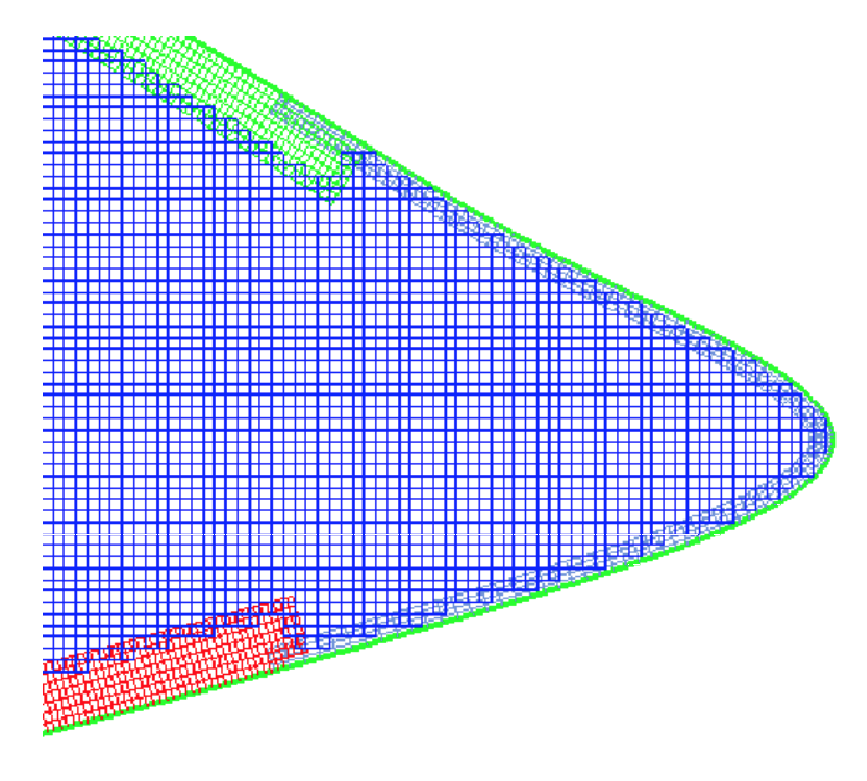
\includegraphics[scale=0.6]{Chapter4/overature_eye}
	\caption{Example of overlapping finite difference grids using Overature. }
	\label{overature_eye}
\end{figure}


In 2007 Heryudono and Braun developed a one-dimensional blinking model of the eye, which included flux conditions of an average supply from the lacrimal gland and drainage due to the puncta \cite{heryudono2007single}. Deng and Driscoll extended this one dimensional model to incorporate a cooling effect, where Chebyshev polynomial approximations were used in the discretization. Through this new model, it was observed that blinking has an effect on the cooling of the tear film \cite{deng2013model,deng2014heat}. Driscoll and Braun then extended these techniques to simulate parabolic flow on an eye-shaped domain \cite{driscoll2018simulation}. As a start, they found numerical solutions for the model
\begin{equation}
\label{driscollPDE}
h_t + \nabla \cdot \vect{q} (h,h_x,h_y)=0, \quad (x,y) \in \mathcal{E}(t),
\end{equation}
where $h$ is the prescribed film thickness and $\vect{q}$ is a known flux function. The domain $\mathcal{E}(t)$ changes with time, as visualized in Figure~\ref{driscoll_eye} and defined in the following section. In particular they examined a second-order thin film analog where
\begin{equation}
\label{thin_film_analog}
\vect{q} = -(A-B h^{-3})\nabla h
\end{equation}
for constants $A$ and $B$ \cite{driscoll2018simulation}. Numerically the PDE is discritized with a Chebyshev polynomial tensor product approximation. In the case of the second order thin film analog with flux (\ref{thin_film_analog}), this led to a solution that was accurate to at least five digits.

In this chapter, we seek to extend this method to solve a fourth order tear film model in a DAE in which the pressure is solved algebraically. In order to meet the computational demands we will use the preconditioned techniques of Chapter 3 to solve this problem. In the following sections, we describe the fourth order tear film model, as well as briefly review how the blinking eye domain $\mathcal{E}(t)$ is transformed from the $[-1,1]^2$. We conclude with a numerical study of our method on the PDE.


\begin{figure}
  \centering
  \includegraphics[scale=0.6]{Chapter4/different_domains}
  \caption{Plot of the subdomains used in \cite{driscoll2018simulation}, where $\mathcal{C}$, $\mathcal{R}(t)$, $\mathcal{E}(t)$ domains are the square, infinite strip and eye-shaped domain. The mappings between the domains are explained in the following section.}
  \label{driscoll_eye}
\end{figure}
	
\section{Model description}

We numerically solve for the height of the tear film $h(x,y,t)$ and pressure $p(x,y,t)$ with the model (\ref{driscollPDE}). Using flux $\bm{q} =  \frac{h^3}{3} \nabla p$ where the pressure is solved algebraically, this produces the model
\begin{align}
\begin{aligned}
h_t &= - \nabla \cdot \lp \frac{h^3}{3} \nabla p \rp, \\
p &= - \ps \nabla^2 h - \pa h^{-3},
\end{aligned} \quad (x,y) \in \mathcal{E}(t)
\label{the_pde}
\end{align}
where $\ps$ represents the ratio of surface tension to viscous forces while $\pa$ is the ratio of van der Waals to viscous forces \cite{braun2015dynamics}. On the boundary we enforce a Dirichlet condition $h=h_0$ as well as flux conditions on $\bm{q}$,
\begin{equation}
\label{normal_conds}
(n \cdot \bm{q})\vert_{\partial \mathcal{E}(t)} = Q_{\text{in}}(x,y,t)+Q_{\text{out}}(x,y,t)
\end{equation}
for prescribed influx and enflux functions $Q_{\text{in}}$, $Q_{\text{out}}$ that incorporate the moving boundary  \cite{li2015computed,heryudono2007single,braun2015dynamics}.
This condition ensures that the total volume of fluid over on $\mathcal{E}(t)$ is conserved over a blink cycle.

%\begin{align}
%\begin{aligned}
%h &= h_{c}, \\
%\bm{n} \cdot \bm{q} &=0
%\end{aligned} \quad (x,y) \in \partial \mathcal{E}(t)
%\label{boundary_conds}
%\end{align}

The domain $\mathcal{E}(t)$ is determined by a pair of two-dimensional transforms. First a fixed square $\mathcal{C}=[-1,1]^2$ is mapped to an infinite strip $\mathcal{R}(t)$ by
\begin{align}
\mathcal{R}(t) = \{(x,y):|y|<\lambda(t)\},
\end{align}
where $-1<\lambda(t)<1$ is a prescribed function. We use the realistic blink motion from \cite{deng2014heat}. The domain $\mathcal{C}$ is mapped to $\mathcal{R}(t)$ via
\begin{align}
	g_x(\hat{x}) = \frac{\gamma \hat{x}}{\alpha^2 - \hat{x}}, \quad g_y(\hat{y}) = \frac{1}{2} (\hat{y}+1)(\lambda(t)+1)-1, \quad (\hat{x},\hat{y}) \in \mathcal{C}
\end{align}
for some $\gamma>0$ and $\alpha \geq 1$.


The domain $\mathcal{E}(t)$ is the image of $\mathcal{R}(t)$ under the conformal map
\begin{align}
f(z) = \tanh(z),
\end{align}
i.e.,
\begin{align}
\mathcal{E}(t) = \{\operatorname{Re}(f(x+iy)),\operatorname{Im}(f(x+iy))|(x,y) \in \mathcal{R}(t)  \}.
\end{align}
If we define $\hat{\nabla}$ to be the gradient in terms of $(\hat{x},\hat{y})$ then
%\begin{align}
%\hat{\nabla} = \frac{\lp \cos(g_y(\hat{y}))+\cosh(g_x(\hat{x})) \rp^2}{1+\cos(g_y(\hat{y}))\cosh(g_x(\hat{x}))} \lp \frac{(\hat{x}^2+\alpha^2)\gamma}{(\hat{x}^2-\alpha^2)^2} \frac{d}{d \hat{x}}, \frac{2}{1+\lambda(t)} \frac{d}{d \hat{y}} \rp.
%\end{align}
\begin{align}
\hat{\nabla} = \frac{1}{|f'(g_x(\hat{x})+i g_y(\hat{x}))|} \lp \frac{(\hat{x}^2+\alpha^2)\gamma}{(\hat{x}^2-\alpha^2)^2} \frac{d}{d \hat{x}}, \frac{2}{1+\lambda(t)} \frac{d}{d \hat{y}} \rp.
\end{align}

Defining $\hat{h}(\hat{x},\hat{y})=h(x,y)$, $\hat{p}(\hat{x},\hat{y})=p(x,y)$, we can determine the tear-film hight and pressure by solving the following index-1 DAE on $\mathcal{C}$:
\begin{align}
\begin{aligned}
\hat{h}_t &= -\frac{1}{3} \hat{\nabla} \cdot (\hat{h}^3 \hat{\nabla} \hat{p}) -\frac{\dot{\lambda}(t)(1+\hat{y})}{\lambda(t)+1} \hat{h}_{\hat{y}} \\
\hat{p} &= - \ps \hat{\nabla}^2 \hat{h} - \pa \hat{h}^{-3}.
\end{aligned}
\end{align}

The normal conditions of (\ref{normal_conds}) greatly simply on $\mathcal{C}$. The influx function $Q_{\text{in}}$ transforms to
\begin{equation}
Q_{\text{in}}(\hat{x},\hat{y},t) = \begin{cases}
Q_{lg}(\hat{x},t) + \dot{\lambda}(t)|f'(g_x(\hat{x})+i g_y(\hat{x}))|(h_0-h_e/2) & \hat{y}=1 \\
0 & \text{otherwise},
\end{cases}
\label{influx_fun}
\end{equation}
where $h_e$ is the thickness of tear fluid under eyelid \cite{heryudono2007single}, and $Q_{lg}$ is the prescribed influx from the lacrimal gland \cite{braun2015dynamics}. For the outflux function we have
\begin{equation}
Q_{\text{out}}(\hat{x},\hat{y},t) = \begin{cases}
Q_{p}(\hat{y},t) & \hat{x}=-1 \\
0 & \text{otherwise},
\end{cases}
\label{out_flux_fun}
\end{equation}
where $Q_{p}(\hat{y})$ describes the efflux from the puncta \cite{braun2015dynamics}.

We define $Q_{lg}$, $Q_{p}$ to be bump functions in space and time. With
\begin{equation}
\step(x,a,b) = 1/2 (1 + \tanh[(4 (a + b - 2 x))/(a - b)])
\end{equation}
we define a indicator like bump function
\begin{equation}
w(x,a,b,h) = \step(x,a,a+h)-\step(x,b-h,b)
\end{equation}
that has support on $[a,b]$ but continuously drops from 1 to 0 in intervals of length $h$. With this bump function and a blink cycle with period $p$, we define
\begin{eqnarray}
\hat{Q_{lg}}(\hat{x},t) &= w(t,0.02,0.1,0.5 p) \exp(((\hat{x}-0.5)/0.25)^2), \label{bumb_funs}  \\
\hat{Q_{p}}(\hat{y},t) &= w(t,0.05,0.1,0.5 p) w(\hat{y},-0.9,0.25,0.9). 
\end{eqnarray}
With target supply and drain volumes $V_s, V_d$ over a blink cycle, we normalize the flux functions (\ref{un_flux}) to define $Q_p,Q_{\lg}$:
\begin{eqnarray}
Q_{lg}(\hat{x},t) &= \frac{V_s}{\int_{0}^{p} \int_{-1}^1 \hat{Q_{lg}} d\hat{x} dt} \hat{Q_{lg}}(\hat{x},t), \\
Q_{p}(\hat{y},t) &= \frac{V_d}{\int_{0}^{p} \int_{-1}^1 \hat{Q_{p}} d\hat{y} dt} \hat{Q_{p}}(\hat{y},t).
\label{un_flux}
\end{eqnarray}
\section{Numerical experiments}
\label{eye_experiments}
For our first experiment, we choose $\pa$ and $\ps$ to be $6.11 \times 10^{-6}$ and $3.09 \times 10^{-6}$, values taken from \cite{braun2015dynamics}. The thickness of the tear film fluid $h_e$ is set to 2 and $V_d=1, V_s=1$.  We solve the model using SNK to solve for the backward time step within ode15s (as described within section~\ref{ode15s_snk}), using the partitioning in Figure~\ref{eye_partition} to better adapt to the features of the tear film height. For each subdomain we use a $35 \times 35$ Chebyshev interpolant approximation.
\begin{figure}
	\centering
	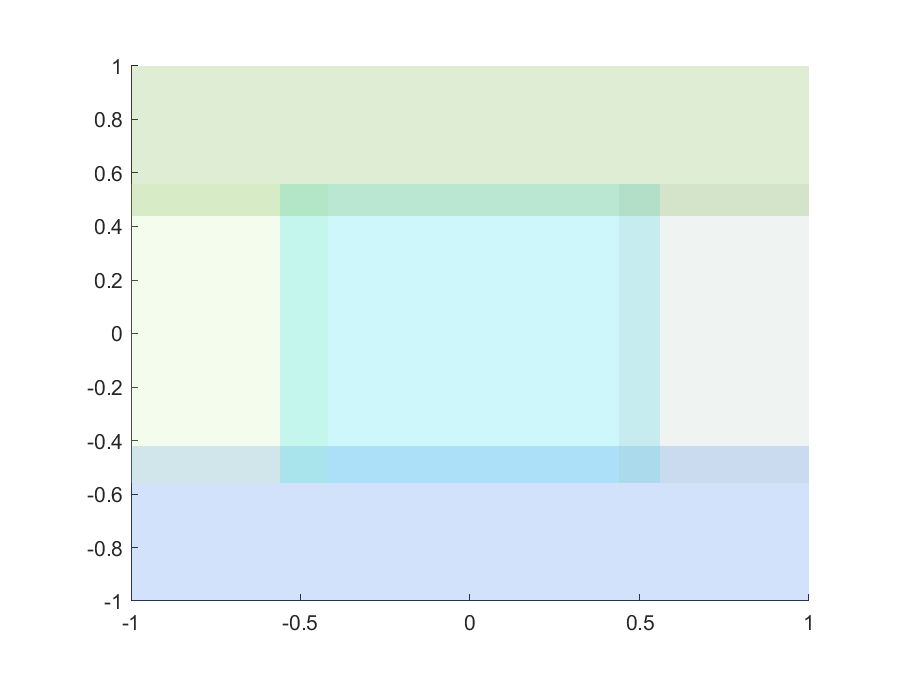
\includegraphics[scale=0.6]{Chapter4/Eye_domains}
	\caption{Plot of subdomains used for blinking eye model.}
	\label{eye_partition}
\end{figure}

We first examine the case of a stationary domain. The boundary conditions of \ref{the_pde} ensure that the volume of the fluid $h(x,y,t)$ is constant over time (in the case of a stationary boundary). As seen in Figure~\ref{eye_volume}, our method maintains a volume that is relatively within $10^{-3}$ of the initial volume, which is indicative of the pointwise error of the numerical solution.

\begin{figure}
	\centering
	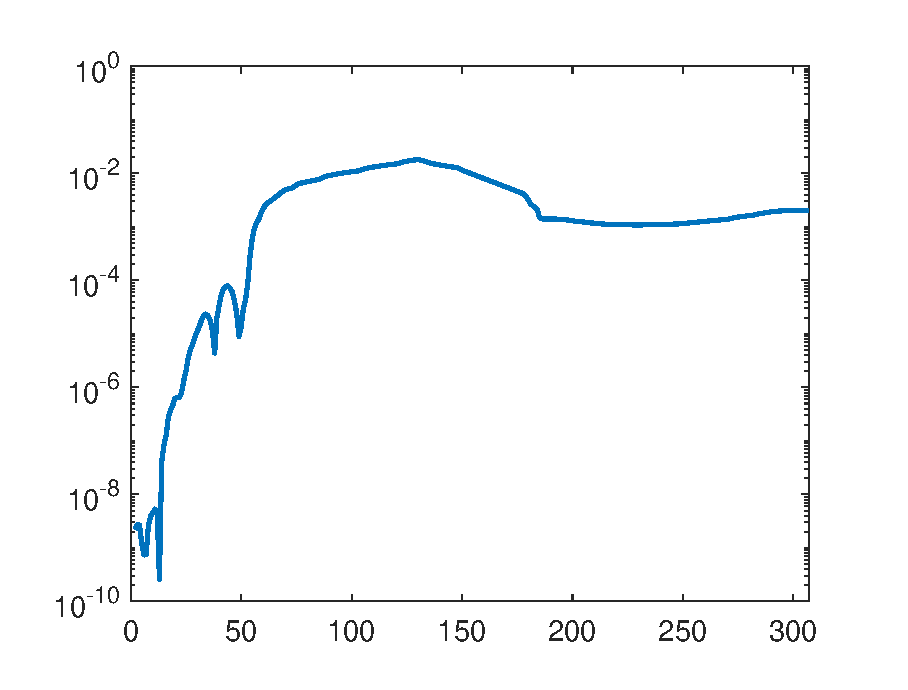
\includegraphics[scale=0.8]{Chapter4/stationary_volume_change}
	\caption{Change of volume of the fluid over time for a stationary boundary. The boundary conditions ensure constant volume over time.}
	\label{eye_volume}
\end{figure}

We now solve the model with the same parameters but with a moving boundary prescribed by the realistic blink motion of \cite{deng2014heat} such that the eye closes 20 percent. With the moving boundary, we expect the volume to be conserved over a blink cycle (that is, it is conserved periodically). After one blink cycle the volume is conserved within a relative difference of $5 \times 10^{-3}$. While the solution was positive throughout the blink cycle, it does become close to zero on the upper left part of the lid half way through the blink cycle as seen in Figure~\ref{tears_02}.

\begin{figure}
	\centering
	\subfloat[Plot of tear film fluid at start of blink cycle.]{
		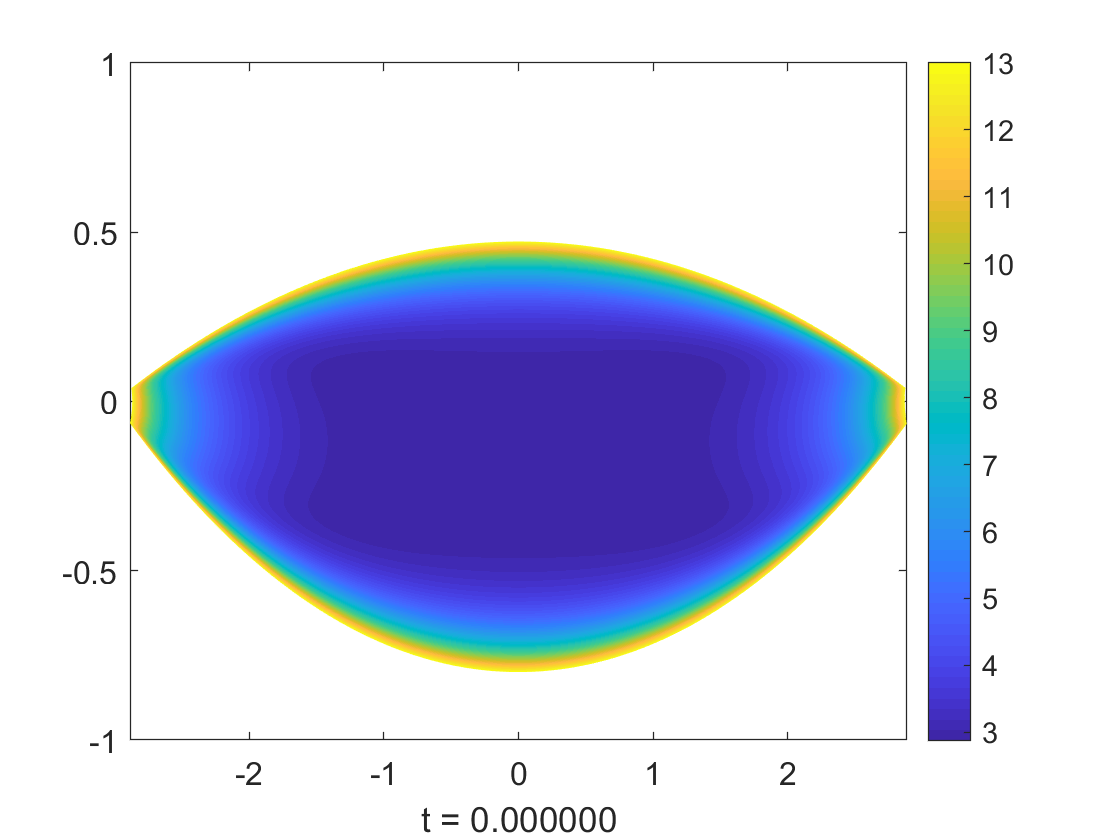
\includegraphics[scale = 0.2]{Chapter4/blink_20_1_0.png}
		\label{tears_02_01}
	}
	\subfloat[Plot of tear film fluid halfway through the blink cycle.]{
		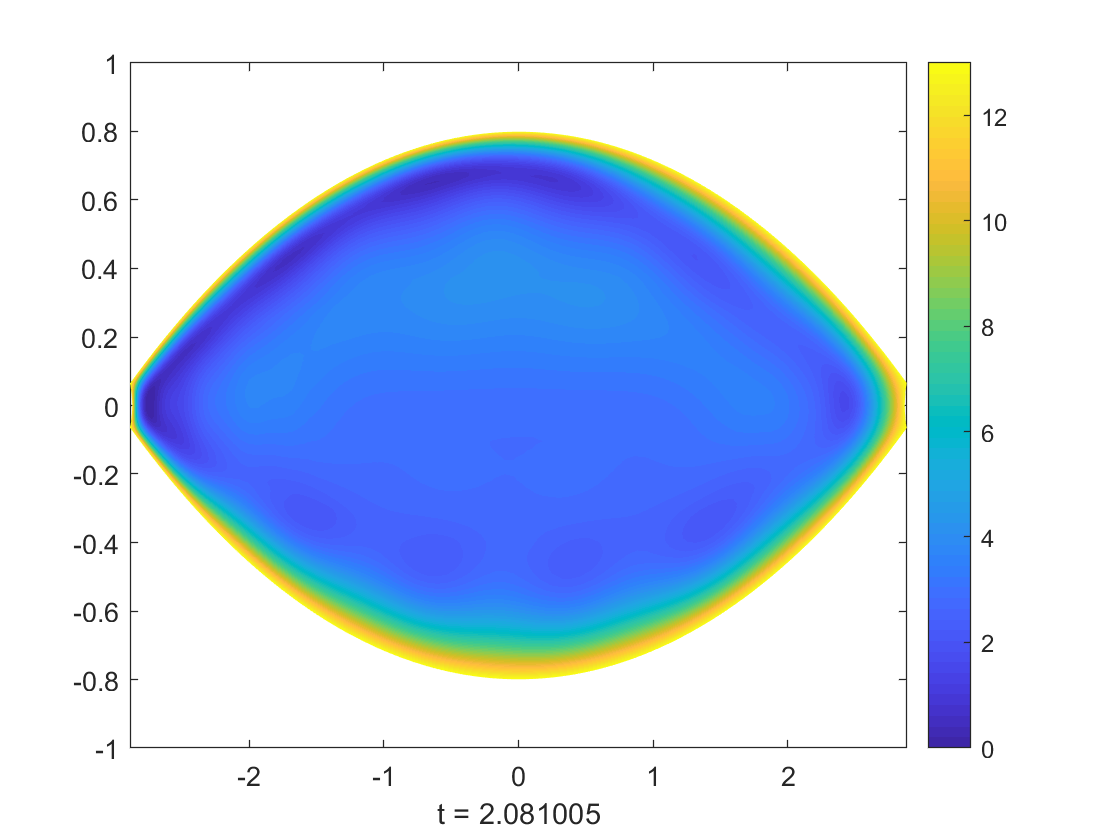
\includegraphics[scale = 0.2]{Chapter4/blink_20_1_0_2.png}
		\label{tears_02_02}
	} 
	\caption{Plot of the tear film hight, where the total influx and outflux is set to 1, and the eye closes 20 percent}
	\label{tears_02}
\end{figure}

This issue becomes more prominent as $V_s,V_d$ increase. As a last experiment we examine the model under more realistic conditions, where the eye closes to 70 percent and $V_s=4,V_d=4$. Numerically we found that this model fails at around 0.7 seconds, as seen in Figure~\ref{broken_tears} since the tear film high becomes negative near the upper left corner. We suspect that this is because the outflux condition (\ref{out_flux_fun}) is overpowering the influx condition (\ref{influx_fun}). This could likely be mitigated by relaxing the bump function (\ref{bumb_funs}) for the puncta fluid efflux, i.e. reducing the height and increasing the width. Further examination and experimentation is needed to find the parameters that give realistic results.

\begin{figure}
	\centering
	\subfloat[Plot of tear film fluid at start of blink cycle.]{
		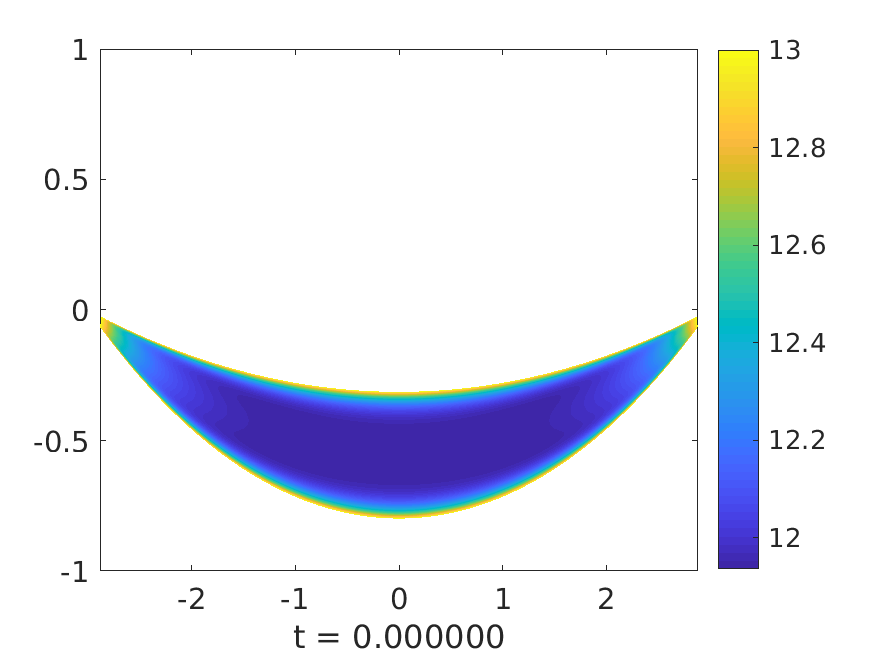
\includegraphics[scale = 0.4]{Chapter4/blinking_eye_broken_start.png}
		\label{broken_tears_0}
	}
	\subfloat[Plot of tear film fluid where it becomes negative.]{
		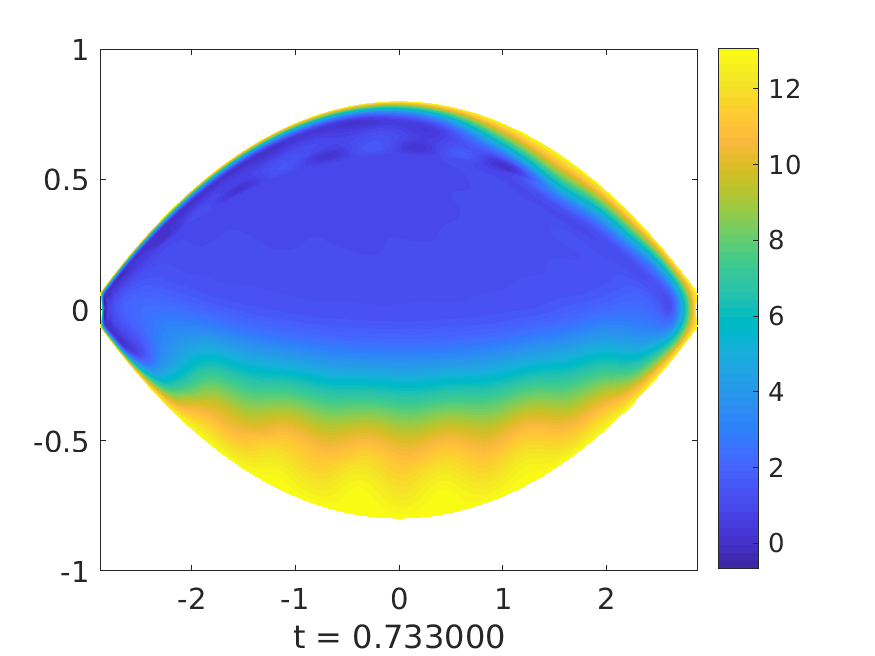
\includegraphics[scale = 0.4]{Chapter4/blinking_eye_broken.png}
		\label{broken_tears_1}
	} 
	\caption{Plot of the tear film hight, where the total influx and outflux is set to 4 and the eye closes 70 percent.}
	\label{broken_tears}
\end{figure}









